\documentclass[conference]{IEEEtran}

% Use of outside images
\usepackage{graphicx} 
% Use text inside euqations
\usepackage{amsmath}

%\usepackage{balance}
\usepackage{float}

\usepackage{hyperref}
\usepackage{nameref}


\floatstyle{plaintop}
\restylefloat{table}

% Correct bad hyphenation here
\hyphenation{op-tical net-works semi-conduc-tor}

\makeatletter
\def\namedlabel#1#2{\begingroup
   \def\@currentlabel{#2}%
   \label{#1}\endgroup
}
\makeatother

\newcommand{\totalCategories}{10}

% Begin the paper here
\begin{document}


% Paper title
% Can use linebreaks \\ within to get better formatting as desired
\title{Sell Prevention and Buy Cure: An Exploration of Indirect Conflicts}

\author{\IEEEauthorblockN{Jordan Ell and Daniela Damian}
\IEEEauthorblockA{University of Victoria,
Victoria, Canada \\ jell@uvic.ca, danielad@csc.uvic.ca}
}

% Make the title area
\maketitle

\begin{abstract}

Awareness techniques have been proposed and studied to aid developer
understanding, efficiency, and quality of software produced. Some of these techniques have focused 
on either \textit{direct} or 
\textit{indirect conflicts} in order to prevent, detect, or resolve these conflicts as they arise
from a result of source code changes. While the techniques and tools for direct conflicts have had
large success, tools either proposed or studied for indirect conflicts have had common issues of
information overload, false positives, and scalability. To better understand these issues, 
we performed a mixed method study involving interviews with 19 developers from 12 commercial and open
source projects, and a survey with 78 responses. Through grounded theory techniques, 
we found: events and conditions which indirect conflicts are likely to occur in
software development, developers prefer to use detection and resolution processes or tools
over those of prevention, developers do not want awareness mechanisms which provide non actionable results,
and that there exists a gap in software evolution analytical tools.

\end{abstract}

\section{Introduction}
\label{sec:intro}

As Software Configuration Management (SCM) has grown over the years, the maturity and norm of parallel 
development has become the standard development process instead of the exception. With this parallel development
comes the need for larger awareness among developers to have ``an understanding of the activities of others
which provides a context for one's own activities''~\cite{Dourish:1992:ACS}. This added awareness
mitigates some downsides of parallel development which include the cost of conflict prevention and resolution. However,
empirical evidence shows that these mitigated losses continue to appear quite frequently and can prove to be a significant
and time-consuming chore for developers~\cite{Perry:2001:PCL}.

Two types of conflicts have attracted the attention of researchers, \textit{direct} and 
\textit{indirect conflicts}. Direct conflicts involve immediate workspace concerns such as developers editing the same
artifact. Tools have been created and studied for direct conflicts
~\cite{Xiang:2008:ERT, Biehl:2007:FVD, Sarma:2009:TIV, Khurana:2009:PFC} with relatively good success and 
positive developer feedback. Indirect conflicts involve source code change influences such as making a sour code change 
which influences behavior negatively in another location in the system (Figure~\ref{fig:ic}). Indirect conflict tools however, have
not shared the same success as direct conflict 
tools~\cite{Sarma:2007:TSA, Holmes:2010:CAR, Trainer:2005:BGT, Servant:2010:CPI, Borici:2012:CHA}.

While indirect conflict tools have shown potential from developer studies, some of the same problems continue
to arise throughout most, if not all tools. The most prevalent issue is that of false positives and information
overload. Through case studies, developers have noted that current indirect conflict tools provide too many 
false positive results, leading to information overload and the tool eventually being
ignored~\cite{Sarma:2007:TSA, Servant:2010:CPI}. A second primary issue is that of dependency identification and
tracking. Many different dependencies have been proposed and used in indirect conflict tools such as method 
invocation~\cite{Trainer:2005:BGT}, and class signatures~\cite{Sarma:2007:TSA} with varying success, but the 
identification of failure inducing changes, other than those which are already identifiable by other means such
as compilers, and unit tests, to these dependencies still remains an issue. Dependency tracking issues are
also compounded by the scale of many software development projects leading to further information overload.
Lastly, social factors such as Cataldo et al.~\cite{Cataldo:2006:ICR} notion of socio-technical
congruence have been leveraged in indirect conflict tools~\cite{Kwan:2011:ESC, Begel:2010:CDE, Borici:2012:CHA}.
However, issues again of information overload, dependencies (in developer organizational structure), and scalability 
come up.

In order to fully understand the root causes of information overload, false positives, and
scalability issues in regards to indirect conflicts, we will take a step back and determine what events occur to
cause indirect conflicts, when they occur, and if conditions exist to provoke more of these events. 
We then set out to understand what mitigation strategies developers currently use as opposed to those created
by academia. Through this exploration, we look to find what can be accomplished moving forward with indirect conflicts
in both research and industry. To accomplish these goals, we ask the following: 

\begin{description}
	\item[RQ1\namedlabel{itm:rq1}{RQ1}] \textit{What events or conditions lead to indirect conflicts?}
	\item[RQ2\namedlabel{itm:rq2}{RQ2}] \textit{What mitigation techniques are used by developers in regards to indirect conflicts?}
	\item[RQ3\namedlabel{itm:rq3}{RQ3}] \textit{What do developers want from future indirect conflict tools?}
\end{description}

We interviewed 19 developers from across 12 commercial and open source projects, followed by a confirmatory survey of 78 
developers, and 5 confirmatory interviews, in order to answer the aforementioned questions. Our findings indicate that: 
indirect conflicts occur frequently and are likely caused by software contract changes and a lack of understanding,
developers tend to prefer to use detection and resolution processes or tools
over those of prevention, developers do not want awareness mechanisms which provide non actionable results, 
and there exists a gap in software evolution analytical tools from the reliance on static analysis resulting in missed
context of indirect conflicts.

\section{Methodology}
\label{sec:meth}

\begin{figure*}[tb!]
\centering
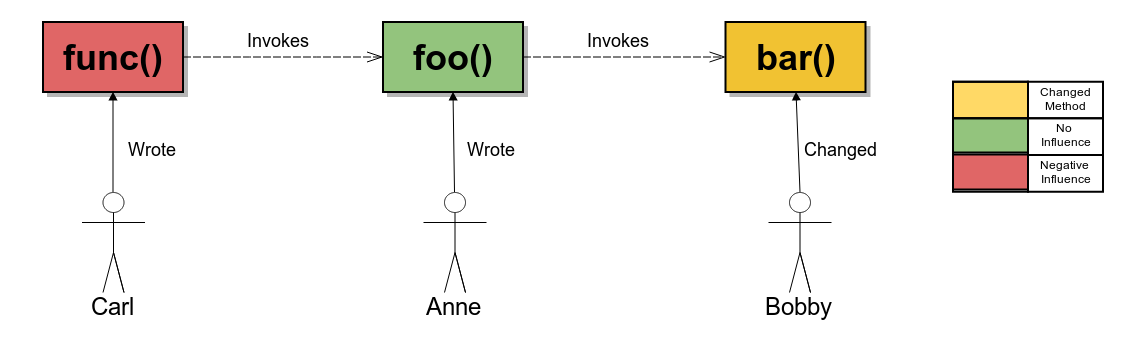
\includegraphics[width=0.9\textwidth]{images/indirect_conflict.png}
\caption{An example of an indirect conflict. Bobby has changed method bar() which has negatively affected method
func() through the chain of invocations.\label{fig:ic}}
\end{figure*}

We performed a a mixed method study in three parts. First, a round of semi-structured interviews were conducted which 
addressed the 3 research questions as mentioned above. Second, a survey was conducted
which was used to confirm and test what was theorized from the interviews on a larger sample size as well as obtain
larger developer opinion of the subject. Third, 5 confirmatory interviews were conducted by re-interviewing original
interview participants to once again confirm and test what had been learned and the results derived by the paper.
Grounded theory techniques were used to analyze the information provided from all three data gathering processes.

\subsection{Grounded Theory}
We approached our study based on grounded theory as described by Corbin and Strauss~\cite{Corbin:1998:SP}.
Grounded theory is a qualitative research methodology that utilizes \textit{theoretical sampling} and
\textit{open coding} to create a theory ``grounded'' in the empirical data. For an exploratory study such as
the ours, grounded theory is well suited because it involves starting from very broad and abstract type questions, and
making refinements along the way as the study progresses and hypotheses begin to take shape. Grounded theory involves
realigning the sampling criteria throughout the course of the study to ensure that participants are able to answer new
questions that have been formulated in regards to forming hypotheses. In our study being presented, data collected from
both interviews and surveys (when open ended questions were involved) was analyzed using open and axial coding. Open coding involves
assigning codes to what participants said at a low sentence level or abstractly at a paragraph or full answer level. These
codes were defined as the study progressed and different hypotheses began to grow. We finally use axial coding it order to
link our defined codes through categories of grounded theory such as context and consequences. 
In Section~\ref{sec:eval}, we give a brief evaluation of our studying using 
3 criteria that are commonly used in evaluating grounded theory studies.

\subsection{Interview Participants}

We selected our interview participants from a large breadth of both open and closed source software development companies
and projects as well as Agile and Waterfall based projects.
The population which participated in our interview came from the following software groups: 
IBM, Mozilla, The GNOME Project, Microsoft Corporation, Subnet Solutions, Ruboss Technology Corporation, 
Amazon, Exporq Oy, Kano Apps, Fireworks Design, James Evans and Associates, and Frost Tree Games. 
Our participants were chosen based on their direct involvement in the actual writing of software for
their respective companies or projects. These participants' software development experience ranged from 3-25 years of experience
with an average of 8 years of experience.
In addition to software development, some participants were also chosen based on their experience with project management
at some capacity.

\subsection{Interview Procedure}

Participants were invited to be interviewed by email and were sent a single reminder email one week
after the initial invitation if no response was made. We directly emailed 22 participants and ended up conducting
19 interviews. Interviews were conducted in person when possible and recorded for audio content only. When in person
interviews were not possible, one of Skype or Google Hangout was used with audio and video being recorded but only
audio being stored for future use. We were pleased with the response rate to our initial invitation emails as
our breadth of participants was rather large, spanning multiple open and closed source, Agile and Waterfall based projects,
and our interview answer saturation~\cite{Guest:2006:SAP} was quite high.

Interview participants first answered a number of structured demographic items, followed by being  
asked to describe various software development experiences regarding our three research questions.
Our three questions were studied by having the interview participants talk about their experiences and opinions in
\totalCategories{} semi-structured research topics.

While each of the \totalCategories{} question categories had a number of starter questions, interviews 
largely became discussions of developer experience and opinion as opposed to direct answers to any specific question.
However, not all participants had strong opinions or any experience on every category mentioned. For these participants, answers 
to the specific categories were not required or pressed upon. We attribute any non answer by a participant to
either lack of knowledge in their current project pertaining to the category or lack of experience in terms of
being apart of any one software project for extended periods of time. We account for these non answers
in our analysis and results as seen in Section~\ref{sec:results}.

\subsection{Survey Participants}

We selected our survey participants from a similar breadth of open and closed source software development 
companies and projects as the interviews participants with two large exceptions. The software organizations
that remained the same between interview and survey were: Mozilla, The GNOME Project, Microsoft Corporation, 
Subnet Solutions, and Amazon.
Participants who took part in the round of interviews were asked to act as a contact point for other 
developers in their team, project, or organization who may be interested
in completing the survey. Aside from this aforementioned list, two other groups of developers were asked to
participate as well, these being GitHub users as well as Apache Software Foundation (Apache) developers. The GitHub
users were selected based on large amounts of development activity on GitHub and the Apache developers
were selected based on their software development contributions on specific projects known to be used heavily
utilized by other organizations and projects.

\subsection{Survey Procedure}

Survey participants were invited to participate in the survey by email. No reminder email was sent as the
survey responses were not connected with the invitation email addresses and thus participants who did respond
could not be identified. We directly emailed 1300 participants and ended with 78 responses
giving a response rate of 6\%. We attribute the low response rate with: the surveys
were conducted during the months of July and August while many participants may be away from their regular positions.
and our GitHub and Apache participants could not be verified as to whether or not they actively support the
email addresses used in the invitations. In addition, the survey was considered by some to be long and require
more development experience than may have been typical of some of those invited to participate.

The created survey~\footnote{http://thesegalgroup.org/people/jordan-ell/iced\_survey/}
was based off of hypotheses created by the round of interviews. The survey
was designed to test these hypotheses and to acquire a larger sample size of developers who may have similar
or different opinions from those already acquired from the interviews. The survey went through two rounds of
piloting. Each pilot round consisted of five participants, who were previously interviewed, completing the survey
with feedback given at the end. Not only did this allow us to create a more polished survey, but it also allowed 
the previously interviewed developers to examine what hypotheses were
formed and what we would be moving forward with.
Each non demographic question was made optional as it was shown 
through the interviews that some questions require more experience from participants than may be provided.

\subsection{Validation}

Following our data collection and analysis, we re-interviewed 5 of our initial interview participants
in order to validate our findings. We confirmed our findings as to whether or not they resonate with 
industry participants' opinions and experiences regarding indirect conflicts and as to their industrial 
applicability. Due to limited time constraints of the interviewed participants, we could only re-interview
five participants. Those that were re-interviewed came from the range of 5-10 years of software development
experience. Re-interviewed participants were given our 3 research questions along with results and main
discussion points, and asked open ended questions regarding their opinions and experiences to validate our 
findings. We also evaluated our grounded theory approach as per Corbin and Strauss'~\cite{Corbin:1998:SP}
list of criteria to evaluate quality and credibility. This evaluation can be seen in Section~\ref{sec:eval}

\section{Results}
\label{sec:results}

We now present our results of both the interviews and surveys conducted in regards to our 3 research questions
outlined in Section~\ref{sec:intro}. We restate each research question, followed by our quantitative and qualitative
results from which we draw our discussion to be seen in Section~\ref{sec:disc}.

\subsection{What events or conditions lead to indirect conflicts?}

From the interviewed participants, 12 developers believe that a large contributing factor to the cause
of indirect conflicts comes from the changing of a software object's contract. Object contracts are, in a sense,
what a software object guarantees, meaning how the input, output, or how any aspect of the object is guaranteed
to work; made famous by Eiffel Software's~\footnote{http://www.eiffel.com/} ``Design by Contract''\texttrademark. 
In light of object contracts, 14 interviewed developers gave examples of indirect conflicts they had experienced
which stemmed from not understanding the far reaching ramifications of a change being made to an object contract
towards the rest of the project. Of those 14, 3 dealt
with the changing of legacy code, with one developer saying ``legacy code does not change because developers 
are afraid of the long range issues that may arise from that change''. Another developer, in regards to changing
object contacts stated ``there are no changes in the input or changes in the output, but the behavior is different''.
Developers also noted that the conflicts that do occur tend to be quite unique from each other and do not necessarily
follow common patterns.

In regards to object contract changes, 9 developers currently working with large scale database applications listed database
schemas as a large source of indirect conflicts while 5 developers that work on either software
library projects or are in test said that methods or functions were the root of their indirect conflict issues. 
7 interviewed developers mentioned that indirect conflicts occur when a major update to an external project, 
library, or service occurs with one developer noting ``their build never breaks, but it breaks ours''. Some
other notable indirect conflict artifacts were user interfaces in web development and full components in component 
base game architecture. 

From the interviewed participants, 11 explained that indirect conflicts occur ``all the time'' in
their development life cycle with a minimum occurrence of once a week, with more serious issues tending
to occur once a month. 65\% of surveyed developers answered that indirect conflicts occur on minimum bi-weekly,
with the majority of developers saying that weekly occurrences are most common.  

12 developers interviewed said that
when a project is in the early stages of development, indirect conflicts tend to occur far more frequently
than once a stable point is reached. Developers said ``At a stable point we decided we are not going to change
[this feature] anymore. We will only add new code instead of changing it.'' and ``the beginning of a project 
changes a lot, especially with agile''. Surveyed developers also added ``indirect conflicts after a release 
depend on how well the project was built at first'', ``[indirect conflicts] tend to slow down a bit after a 
major release, unless the next release is a major rework.'', and ``[indirect conflicts have] spikes during 
large revamps or the implementation of cross-cutting new features.''. Surveyed participants also answered that 
indirect conflicts are more likely to occur before the first major release rather than after at the daily
and weekly occurrence intervals as seen in Table~\ref{tab:often}.

\begin{table*}[tb!]
\begin{center}
\begin{tabular}{| p{7cm} | c | c | c | c | c | c | c |}
\hline
Occurrences & Daily & Weekly & Bi-Weekly & Monthly & Bi-Monthly & Yearly & Unknown \\
\hline
\hline
Early stages of a development & 32\% & 18\% & 4\% & 5\% & 0\% & 5\% & 36\% \\ \hline
Before the first release & 13\% & 29\% & 6\% & 8\% & 1\% & 3\% & 40\% \\ \hline
After the first release & 6\% & 18\% & 8\% & 18\% & 1\% & 5\% & 44\% \\ \hline
Late stages of development & 6\% & 5\% & 5\% & 18\% & 8\% & 12\% & 46\% \\ \hline
\end{tabular}
\end{center}
\caption{Results of survey questions to how often indirect conflicts occur, in terms of percentage
of developers surveyed.\label{tab:often}}
\end{table*}

In terms of organizational structure, surveyed participants answered that as a project becomes larger and more 
developers are added, even to the point that multiple teams are formed, indirect conflicts become more likely to
occur. However, indirect conflicts still occur at a lower number of developers as well with even 43\% of developers
saying they are like to occur in single developer projects.

\subsection{What mitigation techniques are used by developers in regards to indirect conflicts?}

In terms of preventative processes used for indirect conflicts, 3 major components were found.
First, design by contract is heavily used by interviewed developers as a means to avoid indirect conflicts or understand
when they are likely to occur. The use of design by contract here means that developers tend not to change an object's
contract when possible, and that an object's contract is used as a type of documentation towards awareness of the 
software object. One developer stated that ``design by contract was invented to solve this problem and it does it 
quite well'', while another noted that software object contracts do solve the problem in theory, but that doesn't 
mean that problems don't still occur in practice.
Second, 21\% of interview developers mentioned that the add and deprecate 
model is used to prevent indirect conflicts once
the project, feature, or component has reached a stable or mature point.
Add and deprecate meaning instead of editing code, the developer simply clones old code (if needed), and edits the clone
while slowly phasing out the out the old code in subsequent releases or ad needed. This allows other software to 
use the older versions of software objects which remain unchanged, thus avoiding indirect conflicts.
Lastly, pure developer experience was mentioned with 7 developers mentioning that when planning code changes, 
either a very experienced member of the project was involved in the planning and has duties to foresee any 
indirect conflicts that may arise, or that developers must use their personal knowledge to predict where indirect 
conflicts will occur while implementing.

Of the the 37 developers surveyed who could give positive identification of preventative processes for indirect conflicts,
27\% said that individual knowledge of the code base and their impact of code change was used, 59\% mentioned some form of design
by contract or the testing of a methods contract, and 14\% said that add and
deprecate was used in their projects to avoid indirect conflicts.

In regards to catching indirect conflicts, 13 interviewed developers mentioned forms of testing (unit, and integration) 
as the major component of catching indirect conflict issues, subscribing to the idea of ``run the regression and integration 
tests and just see if anything breaks''. The words ``use case coverage'' were constantly being used by developers
when expressing how proper unit and integration tests should be written. Developers expressed that with proper use case coverage, most if
not all indirect conflicts should be caught. 31\% of surveyed developers said build processes (either nightly builds or building the project 
themselves), and others mentioned code reviews while those dealing with a user interface mentioned user complaints from run 
time testing. The surveyed developers confirmed these results with 49\% mentioning forms of testing as the major tool used to 
catch indirect conflicts, 33\% said build processes, while 31\% used work their IDE or IDE plug-ins to catch indirect conflicts.
Surveyed developers also mentioned review process and personal expertise as factors of catching indirect conflicts.

Once an indirect conflict has occurred and developers need to resolve it, 14 developers interviewed said
they checked historical logs to help narrow down where the problem could originate from. Most developers had the mindset of
``Look at the change log and see what could possibly be breaking the feature.''. The log most commonly referred to was the source
code change log to see what code has been changed, followed by build failure or test failure logs to examine errors messages and get time 
frames of when events occurred. Of the developers surveyed, 23\% said they used native IDE tools and 21\% said they use 
features of the language's compiler and debugger in order to solve indirect conflicts. Interestingly, only 13\% of developers 
mentioned a form of communication with other developers in aid to solving these conflicts and only 4\% mentioned the reading 
of formal documentation.

%Very important
Through the processes and tools of prevention, detection, and resolution of indirect conflicts, it is important to note that
most developers ascribe to the idea of ``I work until something breaks'', or taking a curative rather than preventative
approach. This means that while developers do have processes and tool for prevention, they would rather spend their time
at the detection and resolutions stages. One developer noted that preventative processes are ``too much of a burden''
while a project manager said ``[with preventative process] you will spend all you time reviewing instead of implementing''. 

\subsection{What do developers want from future indirect conflict tools?}

When asked about preventative tools, interviewed developers had major concerns that the amount of false positives
provided by the tool which may render the tool useless. Developers said ``this would
be a real challenge with the number of dependencies'', ``it depends on how
good the results are in regards to false positives'', and ``I only want to know if it will break me'', meaning that
developers seem to care mostly about negative impacts of code changes as opposed to all impacts in order to reduce 
false positives and to keep preventative measures focused on real resulting issues as opposed to preventing potential
issues. Overall, developers had little interest in preventative tools or processes.

In terms of catching indirect conflicts, interviewed developers suggested that proper software development processes 
are already in place to catch potential issues such as testing, code review, 
individual knowledge, or static language analysis tools. 68\% of surveyed developers said that they would always
want to be notified about method signature changes as they have a high chance to break the code as opposed to only
23\% who always wanted to be notified on a pre or post condition change and 27\% who want to be notified for a user
interface change. Other change types varied from never being notified to most times being notified, showcasing the
complexity of change types which may or may not negatively affect a project.

When asked about curative tools, developers could only suggest that resolution times be decreased by different means.
Surveyed developers suggested the following improvements to curative tools: 

\begin{itemize}
	\item Aid in debugging by finding which recent code changes are breaking a particular area of code or a test.
	\item Automatically write new tests to compensate for changes.
	\item IDE plug-ins to show how current changes will affect other components of the current project.
	\item Analysis of library releases to show how upgrading to a new release will affect your project.
	\item Built in language features to either the source code architecture (i.e. Eiffel or 
				Java Modeling Language~\footnote{http://www.eecs.ucf.edu/~leavens/JML//index.shtml}) or the compile 
				time tools to display warning messages towards potential issues.
	\item A code review time tool which allows deeper analysis of a new patch to the project allowing the reviewer to see potential 
				indirect conflicts before actually merging the code in.
	\item A tool which is non-obtrusive and integrates into their preexisting development styles without them having to take extra steps.
\end{itemize}

\section{Discussion}
\label{sec:disc}

\textbf{Unwanted Awareness} As we have seen, indirect conflicts are found to be quite a serious problem that occur frequently,
sporadically, and differ greatly from case to case. These conditions pose large issues for the creation of generalizable theories
or tools in regards to indirect conflicts. These underlying complexities are the probable cause of disinterest of software developers
to proposed or implemented tools as discussed in Section~\ref{sec:related}. This inability to generalize is what we believe to be the
leading cause of information overload and false positives in the awareness system, causing developers to eventually ignore 
information being presented to them, rendering the system useless. These false positives are caused by a difference in what
developers consider to be false positives versus what awareness literature considers they are. This disjoint, as will
be seen, is caused by developers only considering events which cause some action to be taken on their part, to be true positives,
where as current awareness understanding would state any event which is related to an individual's 
work~\cite{Herbsleb06collaborationin}~\cite{Cataldo:2008:SCF}, to be true positives.
``You need a good understanding of what the code change is or else you will have a lot of false positives'' said one developer,
showing that not all changes around an object should be reported for awareness.

Developers have been found to have a great understanding of what they need to know about and more importantly what they don't in
their project awareness. To be able to fully understand a developer's awareness intuition, we can see from the results of this paper that
developers only want awareness of an event if the event forces the developer to take some action. In a sense, developers
don't care about what they don't need to account for. ``We would want a high probability of the [reported] change being an issue'', meaning
that the developer only wants the awareness if the item will require action on their part to resolve the issue.
This sense of unwanted or limited awareness is crucial to understand why generalized
awareness techniques of difficult to generalize problems, such as indirect conflicts through generalized changes to 
classes~\cite{Sarma:2007:TSA}, or methods~\cite{Trainer:2005:BGT,Servant:2010:CPI}, often encounter difficulties of false
positives and information overload. 
Developers simply do not want to know about events which effect them, but require no action on their part. 

This unwanted awareness, or limited awareness, seems counter intuitive to current awareness understanding which would state that
being aware of all events in ones surrounding leads to higher productivity or other quality aspects. In theory this is correct,
but as it was found in practice, this is an incorrect assumption. 
In regards to this full awareness, one developer said ``There is no room for this in [our company], as tools are already in place for 
analysis of change[s] and code review takes care of the rest''. Since software developers have limits on their time, awareness of
all events surrounding a developer's work or project is not possible. \textit{Developers prefer to spend their limited time dealing with
the awareness of events which cause them to take some action (changing code, communication, etc) rather than simply being aware
of events occurring around their work which pose no direct threat to the consumption of their time.}

Of course, whether or not this unwanted awareness is the correct path for developers to take is an open question to consider. When
developers encounter a problem which could have been solved by having greater awareness of events which did not directly affect
them initially, we must consider the positive and negative influences of adding this, for now, unwanted awareness. A positive
influence of total, or near total
awareness of events at the developer level, would be the full understanding of a developer's work and environment which comes
with higher quality or understanding of the product. 
A negative influence would be that valuable developer time is spent understanding events which may not directly apply to themselves as opposed to 
producing more output of their own work. This balance between awareness and productivity is found to be a fine line in practice,
however, when given the choice, developers tend to, as previously stated, lean towards less awareness in order to, in their eyes,
be more productive.

\textbf{Prevention versus Cure} We have seen through the results, that developers posses both tools and practices for the prevention,
detection, and resolution of indirect conflicts. We have also seen that through unwanted awareness, and the use of developer time,
that developers tend to prefer working on real issues that have already occurred as opposed to preventing issues of the future which
may never arise. This is neatly explained by the popular adage ``I work until something breaks'' taken by most developers. This mindset
is a clear example of developers taking a curative approach to software development opposed to a preventative approach.
Prevention here refers to taking precautionary steps to stop issues, indirect conflicts, form occurring in the first
place while cure refers to fixing issues as they arise which includes not attempting, or putting little attempt, into preventing
them in the first place.

Two out of the three identified prevention methods taken by developers are simple blanket risk mitigation strategies
accomplished essentially by
not changing code (design by contract, and add and deprecate), while the third is simply developer experience and knowledge. Clearly,
developers are spending little to no time in prevention. Developers do however spend a large amount of time in detection and cure through the
writing of tests and the debugging of issues. In fact, most improvements mentioned by developers in regard to dealing with indirect
conflicts occurred at either the detection or cure levels. Obviously, developers either prefer to spend their time in curative
measures, or do not posses the proper tools to take better action in the preventative stages. ``You're reaction time is much more crucial''
said one developer in that resolution tools are believed to be or larger importance as once issues have occurred, it doesn't
matter what prevention was taken, the issue must simply be resolves as quick as possible now.

The lack of prevention process and tools being used is believed to be due to 2 factors. The first being the identification of dependencies.
Even with an experienced system architect, identifying dependencies and notifying those involved is a daunting task 
which is ignored more than dealt with. The second being the knowledge of when a dependency will fail, also requires vast knowledge
of the product, more than anyone may have. This is compounded by the unique and sporadic nature of indirect conflicts. These 2 factors
are what ultimately have led to the amount of false positives and information overload seen in previous tools. The
abundance of detection and curative process and tools on the other hand shows once again developers willingness to debug
real issues, that maybe even could have been prevented, rather than prevent the issues in the first place. With
this lack of prevention and abundance of curative measures, the question ultimately presented in this area is if 
curative measures are more productive than preventative measures.

Dromey~\cite{Dromey:2003} has raised the debate of prevention versus cure in software development and how difficult a problem it is
to measure. The pros and cons of prevention versus cure we have identified, are similar to those of unwanted awareness,
in that they result in a trade off 
of where time is spent and how productive each side of the argument truly is. If prevention can be shown to be more effective in that
it reduces the number of indirect conflicts or time spent debugging them compared to the time taken to prevent them, should we then
not be moving developers into a more preventative mindset. If curative can be shown to be more effective in that it takes less time
to fix real issues compare to preventing potential ones, should we not be putting more time into automatic debugging, such as
Zeller's Delta Debugging~\cite{Zeller:2002:ICC} or program slicing techniques~\cite{Weiser:1982:PUS}, or automatic test case creation.

A last interesting observation about current curative measures being taken in industry, is that developers view testing of software 
as curative, when one could easily make the argument that it is preventative in that most tests are written to pass originally and
are kept in place to ensure future changes do not cause issues. This mindset may come from the notion that writing tests is originally
thought of as part of normal code writing, meaning that developers see the extra task of test coverage as part of feature implementation.
However, if a test never fails, could it not be said that it is preventing changes from causing it to fail rather than detecting
when failures or indirect conflicts do occur? This may suggest that if, given the write tools, developers may no longer view preventative
measures as a ``burden'' and may be more inclined to take a more balanced preventative approach rather than mostly curative, as
``prevention is the goal'' was commonly said by developers.

This prevention versus cure discussion resides purely on the developer level and should be noted that it may not apply to system
designers, architects, or managerial stakeholders. 
From the project manager's interviewed it was shown that they are heavily favored towards planning and 
prevention (even though their prevention may be on more abstract levels than developers actually need) while leaving the curative
approaches to their developers. The prevention versus cure debate may have different outcomes depending on what level of abstraction
is being viewed in research.

%mature point, static analysis
\textbf{Gap in Software Evolution Analysis} Indirect conflicts are more likely to occur,
from developer opinion, before a mature point is reached in the project's evolution. ``Once you get the API stable, people are 
better at communicating changes in regards to dependency concerns.''(This mature point may stem from a major release,
end of an iteration, a new feature being released or any point considered stable and reliable) However, this context of a 
mature point, as well as any other
potential contextual attributes, are rarely identified or accounted for in regards to indirect conflicts. Developers have said
that different change types may occur at different rates throughout a project's life time and that this
may drastically effect the outcomes of indirect conflict tools or processes.

A deeper understanding of what context indirect conflicts occur in seems to be more of a success factor to indirect conflict
research than may have been previously thought. Static analysis may be useful in regards to indirect conflict context in that we
could identify trends surrounding the mature points of previous projects in order to give a better understanding of what it
means for a project to be pre or post mature point, which could affect the outcome of indirect conflict understanding.
Fluri et al.~\cite{Fluri:2007:CDT} uses static analysis and abstract syntax trees to be able to determine what types of source code
changes occur at a given point in time which could be used for determining such a context of mature points.

This added level of context, through the notion of a mature point, 
would add to the prevention versus cure debate as previously discussed. Prevention may be a better
choice once a project has reached a mature point as the code base becomes more stable and source code changes become more dangerous
to the quality of the project. Curative measures may be a better choice before a mature point as code churn can be higher which
causes more bugs than can be prevented. These possibilities existing, it may be imperative to discover more of project stability
and the mature point in order to fully understand the nature of indirect conflicts and their context.

While this added sense of understanding is important to indirect conflicts, contextual attributes of a project's current progress
or measures of performance are often more synonymous with project management
rather than software developers themselves. An understanding of a project's evolution, a mature point being reached as an example,
may pose as a more useful tool for project management rather than developers. This more abstract tendency of indirect
conflict occurrences may add even more power to project management for evaluation of progress, code stability, and code reviews.

Aside from context, dependency identification and tracking is a key missing component of
indirect conflict analysis due to the weaknesses of static analysis. The gap in this identification comes from software and 
organizational structures of software teams. Between increased modularization (multiple sub projects or repositories), 
cross language dependencies, and languages which do not lend themselves to static analysis, static analysis tools have 
become quite limited in identifying and tracking dependencies where they were once strong.

Relational database schemas are one of the highest sources of indirect
conflicts found in their projects, ``it breaks stuff all over the place'',
yet we know from Maule et al.~\cite{Maule:2008:IAD} that relational database schemas have 
been scarcely researched in terms of indirect conflicts. This falls in with our previous understanding of cross language
dependency tracking in that database schemas are independent of languages which may be on the receiving end of their output.

These increases of complexity in software products has left quite a gap in dependency identification and tracking which 
has lead to some of the deficiencies of indirect conflict research.


\subsection{Implication for Research}
\label{sec:implr}

\textbf{Prevention versus Cure}
The largest implication for future research found in this paper is the need for continued study of the open question
``Which of prevention or cure is more effective for software development and indirect conflicts?''. This simple question will undoubtedly 
produce extremely complex answers. With software developers focusing their current efforts on curative measures, for
indirect conflicts, suggests
that while it may not be the most effective, it may be the easiest road for developers to take. This may be the path of
least resistance, but it may not be optimal. Software engineering as a whole should strive to answer this question or
provide more insight into possibilities, as its answer may determine many future actions taken by the research community.

Recommendations towards the study of prevention versus cure involve the examination of formal processes and tools used
by industry professionals with measurements of efficiency and effectiveness, similar to the work of
Tiwana~\cite{Tiwana:2008:ICD} in coordination tools. With these studies, we may find insight into the correct balance
of prevention versus cure, thus being able to increase developer productivity as well as identify more gaps in theory 
versus practice which may lead to improved tools or the abandoning of existing ones as was shown with UML~\cite{Petre:2013:UP}.

\textbf{Awareness Theory to Model Real World}
A second implication for research more directly related to awareness, is the need to further characterize the
mismatch between awareness approaches and tools as developed in the research community and awareness needs as perceived
by industry.
As was identified in the previous discussion, while current understanding suggests that awareness of all events related to ones work
produces a more coherent understanding of a person's environment, developers find this to be overly time consuming
to the point where they only want to be aware of events which require action on their part. This difference, of what 
should be and what is, should be further understood to combat future potential failures in
tool development or theories attempted to be used in practice.

\subsection{Implication for Tools}
\label{sec:implt}

\textbf{Give Developers What They Want}
The direct implication this research has on tool creation is that of current adoption among developers. As was stated,
developers are more keen to invest their time at the detection and cure / resolution stages of indirect conflicts. That being 
said, focus at these two stages for tool developer will lead to larger adoption among developers.
It should be noted here that detection must come with an almost zero rate of false positives as
current tools (unit and integration and user testing), while they may not have 100\% recall, have almost 100\% precision.

\textbf{Stronger Source Code Analysis}
The more indirect implication of this research on tool creation is that of improving existing tools. While not all existing
tools are used for indirect conflicts alone (automatic debugging~\cite{Zeller:2005:WPF}, unit tests, etc), most of these tools
have need for rapid expansion, according to developers, for dealing with indirect conflicts. The ability to have unit tests
automatically written for a given software object's contract, the ability to find a change  in an external project
which has broken a developer's own project, or any automation of the existing detection and resolution stages of indirect
conflicts are what developers currently seek. But of course, most of these implications rely on the improvement of 
static analysis tools.

These tool implications themselves imply the need of further development of static analysis tools. Static 
analysis lays at the heart of most if not all stages of indirect conflict research. We must be able to track and manage
software dependencies across the new landscape of software development that is multiple projects, repositories, and cross
language support. These improvements will allow the further development of both current and future indirect conflict
tools.

\section{Evaluation}
\label{sec:eval}

From the re-interviewed participants, we found extremely positive feedback regarding both our results and major discussion
points. Participants often had new stories and experiences to share once they had heard the results of this paper which
confirmed the findings and often were quite shocked to hear the results as they did not usually think about their actions
as such but then realized the results held true to their daily actions for better or worse.

As per grounded theory research, Corbin and Strauss list ten criteria to evaluate quality and credibility~\cite{Corbin:1998:SP}.
We have chosen three of these criteria and explain how we fulfill them.

{\bfseries Fit.} ``Do the findings fit/resonate with the professional for whom the research was intended and the participants?'' This
criterion is used to verify the correctness of our finding and to ensure they resonate and fit with participant opinion. It is also
required that the results are generalizable to all participants but not so much as to dilute meaning. To ensure fit, during interviews
after participants gave their own opinions on a topic, we presented them with previous participant opinions and asked them to comment
on and potentially agree with what the majority has been on the topic. Often the developers own opinions already matched those of
the majority before them and did not necessarily have to directly verify it themselves.

As added insurance, we conducted 5 post results interviews with developers to once again confirm our results, and discussions. These
procedures can be seen in Section~\ref{sec:meth}.

To ensure the correctness of the results, we also linked all findings in Section~\ref{sec:results} to either a majority of agreeing
responses on a topic or to a large amount of direct quotes presented by participants.

{\bfseries Applicability or Usefulness.} ``Do the findings offer new insights? Can they be used to develop policy or change practice?''
Although our results may not be entirely novel or even surprising, the combination of said results allowed us to discover the
the disjoint between theoretical awareness and practical awareness regarding indirect conflict tools as well as provide more
insight into the debate of prevention versus cure in software development. Given how many indirect conflict tools are left with the same common
issues, we believe that these findings will help researchers focus on what developers want and need moving into the future more than has
been possible in the past. These finding set a course of action for where effort should be spent in academia to better benefit industry.

10 of the 78 participants who were surveyed sent direct responses to us asking for any results of the research to be sent directly to
them in order to improve their indirect conflict work flows. 7 of the 19 participants interviewed expressed interest concerning any possible
tools or plans for tools inspired by this research as well. The combination of academia relatability and direct industry interest 
in our results help us fulfill this criterion.

{\bfseries Variation.} ``Has variation been built into the findings?'' Variation shows that an event is complex and that any findings
made accurately demonstrate that complexity. Since interviewed participants came from such a diverse set of organizations, 
software language knowledge, and experience the variation naturally reflected the complexity. Often in interviews and surveys, participants
expressed unique situations that did not fully meet our generalized findings or on going theories. In these cases, we worked in the specific
cases which were presented as boundary cases and can be seen in Section~\ref{sec:results} as some unique findings or highly
specialized cases. These cases add to the variation
to show how the complexity of the situation also resides in a significant number of unique boundary situations as well as the complexity
in the generalized theories and findings.

\section{Related Work}
\label{sec:related}

Since this paper has covered a wide spectrum in regards to indirect conflicts (prevention, detection, resolution, process, and tools), there
exists a large body of work in which to draw from regarding indirect conflicts. While some of the previous literature may not deal explicitly
in the notion of indirect conflicts, lessons learned from topics in awareness, direct conflict detection, and debugging are presented.

Many indirect conflict tools have been created, tested, and published. Sarma et al.~\cite{Sarma:2007:TSA} created Palantir, 
which can both detect potential indirect conflicts, at the class signature level, and alert developers to these conflicts. 
Palantir represented one of the first serious attempts at aiding developers towards indirect conflicts. Holmes et 
al.~\cite{Holmes:2010:CAR} take it one step further with their tool YooHoo, by detecting fine grained source code changes, 
such as method return type changes, and create a taxonomy for different types of changes and their proneness to cause 
indirect conflicts. This tool and its taxonomy had a severely reduced false positive rate, however, the true positives 
detected may already be detectable by current tools such as compilers and unit testing. The tool Ariadne~\cite{Trainer:2005:BGT} 
creates an environment where developers can see how source code changes will affect other areas of a project at the 
method level, using method call graphs, showing where indirect conflicts may occur. This type of exploratory design has 
been used often in the visualization of indirect conflict tools, allowing developers a type of search area for their development
needs. Another indirect conflict tool, CASI~\cite{Servant:2010:CPI}, utilizes dependency slicing~\cite{Bajracharya:2009:SIS} 
instead of method call graphs to provide an environment to see what areas of a project are being affected by a source code change. 
Most of these tools have all shown to have the same common difficulties of scalability, false positives, and information overload, 
which were explored in this paper. Our own tool 
Impact!~\footnote{University of Victoria Computer Science Technical Paper: DCS-351-IR} also suffered these same fates.

Since Cataldo et al.~\cite{Cataldo:2006:ICR} have shown that socio-technical congruence can be leveraged to improve task completion
times, many indirect conflict tools support the idea of a socio-technical congruence~\cite{Kwan:2011:ESC} in order to help
developers solve their indirect conflict issues through social means~\cite{Begel:2010:CDE}~\cite{Borici:2012:CHA}. 
Begel et al.~\cite{Begel:2010:CDE} created Codebook, a type of social developer network related directly to source code
artifacts, which can be used to identify developers and expert knowledge of the code base. Borici et al.~\cite{Borici:2012:CHA}
created ProxiScientia which used technical dependencies between developers to create a network of coordination needs.
Socio-technical congruence however, is largely unproven in regards to its correlation to
software quality~\cite{Kwan:2011:SCE} and again the problems of scalability and information overload become a factor.

For developer interest in regards to software modifications, Kim~\cite{Kim:2011:ESA} found that developers wanted to know whose 
recent code changes semantically interfere with their own code changes, and whether their code is impacted by a code change.
Kim conducted several focus groups as well as web surveys to determine these results. These areas of interest resonate with what was
found in this paper. Developers want to know when a code change is going to interfere with their work in a potentially negative way and
require action on the developer's half.  Kim
also found that developers are concerned with interfaces of objects and when those interfaces change, similar to the object contracts that
were found in this paper. Finally, Kim also identified the same issues towards information overload through false positives with developers
noting ``I get a big laundry list... I see the email and I delete it''.

In a case study of impact awareness, de Souza et. al.~\cite{deSouza:2008:ESS} found that developers use their personal knowledge of the
code base to determine the impact of their code changes on fellow developers, teams, and projects. This corresponds with the findings of
preventative measures we have found in that some human interaction or knowledge is required in preventing indirect conflicts along with
development processes.

In a study regarding static analysis tools, Johnson et. al~\cite{Johnson:2013:WDS} found similar conclusions towards the
ill fit of current static analysis to current development practices. Not being designed properly to fit current development work
flow, and the over abundance of false positives were shown to be factors of developer non-use. 

Hattori et. al.~\cite{Hattori:2012:ICG} found, through qualitative user studies, that developers tend to use the bare amount of communication
towards other developers in order to solve direct conflicts, and take the same approach of only communicating once a conflict has arose. This
resonates with ``I work until something breaks''. Hattori et. al. also show that with direct conflicts, the
sooner preemptive information if available to developers the more they will communicate and either avoid or easily solve their code merges.
This is the situation many indirect conflict tools have strived for. In terms of communication, Bolici et. al~\cite{Bolici:2009} give the 
possibility of developer stigmergy as the reason that developers do not need to explicitly communicate with each other about issues. The idea
that developers use artifacts left behind by other developers to solve their issues could play a large role in a lack of formal communication.
Blincoe et al.~\cite{Blincoe:2013:UCC} also found, through data mining techniques, a subset of events related to awareness 
which occur that developers will communicate about as opposed to all awareness events. This again confirms our understanding that developers
only care about certain events which require some action on their part.

While not specifically developed with indirect conflicts in mind, Zeller's delta debugging techniques~\cite{Zeller:2005:WPF}, 
can be applied to solving indirect conflict issues. Zeller gives automated techniques for identifying failure-inducing
changes (as well as other failure causing components) of the software project in order to isolate and debug some issue. These practices fit
with the idea that developers wait for something to go wrong, then wish to fix the issue as fast as possible. Program slicing~\cite{Xu:2005:BSP}
has also been extensively studied in order to aid in debugging in manual or automated techniques.

\section{Conclusions}
\label{sec:conc}

Indirect conflicts are a significant issue with real world development, however, many proposed techniques and tools to mitigate
losses in this realm have been unsuccessful in attracting major support from developers. Based on our qualitative study involving
19 interviewed developers from 12 organizations as well as 78 surveyed developers, we have provided characterization of indirect conflicts,
current developer work flow surrounding indirect conflicts, and what direction any future tools should follow in order to aid developers
in their work flow with indirect conflicts.

We have shown through the findings of RQ1 why indirect conflicts occur, when indirect conflicts are more likely to
occur, as well as what types of software objects are susceptible to these conflicts. Results of RQ2 have shown
how developers in industry currently handle the prevention detection and solving of indirect conflicts. And Lastly, findings of RQ3
have provided a foundation as to why past techniques and tools have had low adoption rates and where
researchers should focus their current and future efforts in handling indirect conflicts. 

We have shown the disjoint of current awareness understanding versus the practical
awareness needs found in industry. This disjoint, caused by the difference of academic and practical understanding in awareness needs,
ultimately lead to tools with information overload and false positive issues. The debate of prevention versus cure has been presented along with
the industrial tendency towards curative measures. While a curative approach may be favored by developers, further research is needed
to fully asses the positive and negative influences of prevention versus cure for productivity and quality concerns. Finally, we have shown
the gap of analytical evolution tools needed for dependency identification and indirect conflicts. This gap, unless addressed, may prevent
future industrial adoption of tools produced by academia for lack of fit in industrial needs.

\section{Acknowledgments}

We sincerely thank all participants who were willing to be interviewed or who participated
in completing our survey. We thank these people for taking time out of their day to participate and for
sharing their developer experience with us.

\bibliographystyle{IEEEtran}
%\balance
\bibliography{paper}

% End of the paper
\end{document}
